\documentclass[nobib]{tufte-handout}

%\\geometry{showframe}% for debugging purposes -- displays the margins

\newcommand{\bra}[1]{\left(#1\right)}
\usepackage{amssymb}
\usepackage{hyperref}
\usepackage{pgfplots}
\usepackage[activate={true,nocompatibility},final,tracking=true,kerning=true,spacing=true,factor=1100,stretch=10,shrink=10]{microtype}
\usepackage{color}
\usepackage{steinmetz}
\usepackage{placeins}
% Fixes captions and images being cut off
\usepackage{marginfix}
\usepackage{array}
\usepackage{tikz}
\usepackage{amsmath,amsthm}
\usetikzlibrary{shapes}
\usetikzlibrary{positioning}
\usepackage{listings}
\usepackage{caption}
\DeclareCaptionFont{white}{\color{white}}
\DeclareCaptionFormat{listing}{\colorbox{gray}{\parbox{\textwidth}{#1#2#3}}}
\captionsetup[lstlisting]{format=listing,labelfont=white,textfont=white}

% Set up the images/graphics package
\usepackage{graphicx}
\setkeys{Gin}{width=\linewidth,totalheight=\textheight,keepaspectratio}
\graphicspath{{.}}

\title{Notes for ECE 36800 - Data Structures and Algorithms}
\author[Shubham Saluja Kumar Agarwal]{Shubham Saluja Kumar Agarwal}
\date{\today}  % if the \date{} command is left out, the current date will be used

% The following package makes prettier tables.  We're all about the bling!
\usepackage{booktabs}

% The units package provides nice, non-stacked fractions and better spacing
% for units.
\usepackage{units}

% The fancyvrb package lets us customize the formatting of verbatim
% environments.  We use a slightly smaller font.
\usepackage{fancyvrb}
\fvset{fontsize=\normalsize}

% Small sections of multiple columns
\usepackage{multicol}

% For finite state machines 
\usetikzlibrary{automata} % Import library for drawing automata
\usetikzlibrary{positioning} % ...positioning nodes
\usetikzlibrary{arrows} % ...customizing arrows
\tikzset{node distance=2.5cm, % Minimum distance between two nodes. Change if necessary.
    every state/.style={ % Sets the properties for each state
    semithick,
    fill=gray!10},
    initial text={}, % No label on start arrow
    double distance=2pt, % Adjust appearance of accept states
    every edge/.style={ % Sets the properties for each transition
    draw,
    ->,>=stealth', % Makes edges directed with bold arrowheads
    auto,
    semithick}}
\let\epsilon\varepsilon

% These commands are used to pretty-print LaTeX commands
\newcommand{\doccmd}[1]{\texttt{\textbackslash#1}}% command name -- adds backslash automatically
\newcommand{\docopt}[1]{\ensuremath{\langle}\textrm{\textit{#1}}\ensuremath{\rangle}}% optional command argument
\newcommand{\docarg}[1]{\textrm{\textit{#1}}}% (required) command argument
\newenvironment{docspec}{\begin{quote}\noindent}{\end{quote}}% command specification environment
\newcommand{\docenv}[1]{\textsf{#1}}% environment name
\newcommand{\docpkg}[1]{\texttt{#1}}% package name
\newcommand{\doccls}[1]{\texttt{#1}}% document class name
\newcommand{\docclsopt}[1]{\texttt{#1}}% document class option name

% Define a custom command for definitions and biconditional
\newcommand{\defn}[2]{\noindent\textbf{#1}:\ #2}
\let\biconditional\leftrightarrow

\begin{document}

\maketitle

\begin{abstract}
    These are lecture notes for spring 2024 ECE 36800 at Purdue. Modify, use, and distribute as you please.
\end{abstract}

\tableofcontents

\section{Course Introduction}
Provides insight into the use of data structures. Topics include stacks, queues
and lists, trees, graphs, sorting, searching, and hashing. The learning
outcomes are:
\begin{itemize}
    \item Advanced programming ideas, in practice and in theory
    \item Data structures and their abstractions: Stacks, lists, trees, and graphs
    \item Fundamentals of algorithms and their complexities: Sorting, searching, hashing,
          and graph algorithms
    \item Problem-Solving
\end{itemize}
\pagebreak

\section{Introduction to Data Structures \& Algorithms}
Data Structures are methods of organizing information for ease of manipulation.
Examples:
\begin{enumerate}
    \item Dictionary
    \item Check-out line or queues
    \item Spring-loaded plate dispenser or stacked
    \item Organizational Chart or tree
\end{enumerate}
These are associated with methods known as algorithms to be manipulated\\
Algorithms are methods of doing something.
Examples:
\begin{enumerate}
    \item Multiplying two numbers
    \item Making a sandwich
    \item Getting dressed
\end{enumerate}
The topics of interest within them are:\\
\begin{itemize}
    \item Correctness
    \item Efficiency in time and space
\end{itemize}
\section{Time Complexity Analysis}
The questions to be asked about an algorithm are the following:
\begin{itemize}
    \item Is it correct?
    \item Is it as fast as possible?
    \item How many machine instructions (in terms of n) does it take?
\end{itemize}
Let us take the following algorithm to add the numbers form 1 to n:
\begin{lstlisting}
    total = 0;
    for (i=1:n)
        total = total + i;
    return total
\end{lstlisting}
The cost will be:\\
\begin{table}
    \centering
    \begin{tabular}{c|c|c}
        Cost  & Frequency & Function                     \\
        \hline
        $C_1$ & 1         & Assign initial value         \\
        $C_2$ & n+1       & For loop iterations and exit \\
        $C_3$ & n         & Number additions             \\
        $C_4$ & 1         & Return value                 \\
    \end{tabular}
\end{table}
\FloatBarrier
The total is then:\\
\begin{align*}
    C_1*1+C_2(n+1)+C_3(n)+C_4(1) & = (C_2+C_3)n+ (C_1+C_2)+C_4
\end{align*}
However the $O(n)$ will only be n, as the constants and coefficients of these will be deprecated, as we will come to understand in more detail as this topic continues.\\
Let us take another example of some code that has a
\begin{align*}
    T(n)                                     & = n^2 + 10^7n+10^{10}                                \\
    T(10^{11})                               & = 10^{22} + 10^{18}+ 10^{10}                         \\
    T(2*10^{11})                             & = 4*10^{22} + 2*10^{18}+ 10^{10}                     \\
    \implies \frac{T(2*10^{11})}{T(10^{11})} & \approx 4 = \left(\frac{2*10^{11}}{10^{11}}\right)^2
\end{align*}
This goes to show that this algorithm has an $O(n) = n^2$, and all coefficients and lower order terms that are a part of the complexity are largely irrelevant for large n values.
This is why this is called \textbf{asymptotic notation}.\\
Another example of a simple algorithm is
\begin{lstlisting}
    total = 0;
    for (i=1:n):
        if (((i*i%3)==0)||((i*i%7)==0)):
            total = total+i*i;
    return total;
\end{lstlisting}
Which has a cost table that looks like the following:\\
\begin{table}
    \centering
    \begin{tabular}{c|c|c}
        Cost  & Frequency                                                                                  & Function                     \\
        \hline
        $C_1$ & 1                                                                                          & Assign initial value         \\
        $C_2$ & n+1                                                                                        & For loop iterations and exit \\
        $C_3$ & n                                                                                          & Number of $i\%3$ comparisons \\
        $C_4$ & $n - \lfloor \frac{n}{3} \rfloor  $                                                        & Number of $i\%7$ comparisons \\
        $C_5$ & $\lfloor \frac{n}{3} \rfloor + \lfloor \frac{n}{7} \rfloor - \lfloor \frac{n}{21} \rfloor$ & Number of additions          \\
        $C_6$ & 1                                                                                          & Returning value              \\
    \end{tabular}
\end{table}
It can be noted that $O(n) = n$ for this function, despite all the other complexities in the algorithm. However, it is important to know how to calculate $T(n)$ as well.\\
Now, let us look at something more complicated, matrix multiplication of two lower triangular matrices.
\begin{lstlisting}
    for (i=1:n):
        for (j=1:i):
            C_ij = 0;
            for (k=j:i):
                C_ij = C_ij+A_ik*B_kj
    return C
\end{lstlisting}
This has a cost table that looks like the following:
\begin{table}
    \centering
    \begin{tabular}{c|c|c}
        Cost  & Frequency                                        & Function                    \\
        \hline
        $C_1$ & n+1                                              & First loop                  \\
        $C_2$ & $\sum_{i=1}^{n} (i+1)$                           & Second loop                 \\
        $C_3$ & $\sum_{i=1}^{n} \sum_{j=1}^{i} 1 $               & Number of assigns           \\
        $C_4$ & $\sum_{i=1}^{n} \sum_{j=1}^{i} (i-j+2) $         & Third loop                  \\
        $C_5$ & $\sum_{i=1}^{n} \sum_{j=1}^{i} \sum_{k=j}^{i} 1$ & Number of assigns to matrix \\
        $C_6$ & 1                                                & Returning value             \\
    \end{tabular}
\end{table}
Finally, we can analyze an example that has logarithmic complexities.
\begin{lstlisting}
    i=2;
    k=0;
    while (i<n){
        i=i*i;
        k=k+1;
    }
    return i;
\end{lstlisting}
Which has a cost table that looks like the following:\\
\begin{table}
    \centering
    \begin{tabular}{c|c|c}
        Cost  & Frequency                          & Function                        \\
        \hline
        $C_1$ & 1                                  & Assign i                        \\
        $C_2$ & 1                                  & Assign k                        \\
        $C_3$ & $\lceil \log_2(\log_2(n))\rceil+1$ & Number of while loop iterations \\
        $C_4$ & $\lceil \log_2(\log_2(n))\rceil $  & number of assigns of i          \\
        $C_5$ & $\lceil \log_2(\log_2(n))\rceil$   & Number of k assigns             \\
        $C_6$ & 1                                  & Returning value                 \\
    \end{tabular}
\end{table}

It can be noted that if line three was instead changed to\\
\begin{lstlisting}
    while (i<=n){
\end{lstlisting}
The table will instead be:\\
\begin{table}
    \centering
    \begin{tabular}{c|c|c}
        Cost  & Frequency                            & Function                        \\
        \hline
        $C_1$ & 1                                    & Assign i                        \\
        $C_2$ & 1                                    & Assign k                        \\
        $C_3$ & $\lceil \log_2(\log_2(n+1))\rceil+1$ & Number of while loop iterations \\
        $C_4$ & $\lceil \log_2(\log_2(n+1))\rceil $  & number of assigns of i          \\
        $C_5$ & $\lceil \log_2(\log_2(n+1))\rceil$   & Number of k assigns             \\
        $C_6$ & 1                                    & Returning value                 \\
    \end{tabular}
\end{table}
\FloatBarrier
As the loop break condition changed from $i\geq n$ to $i\geq n+1$ by simply changing.
\section{Insertion and Shell Sort}
Sorting is necessary to process items in sorted order. It speeds up the
location of items, finding identical items, etc. \\ It is good to know that in
real life, what is sorted is in fact the pointers of these structs, as the
movement of structs have higher memory requirements.
\subsection{Insertion Sort}
Inserts an item into a sorted array. Compares the item with items in the sorted
array, and if they are in the incorrect order, they are swapped. This is
continued until everything has been successfully sorted.\\ The code to sort $n$
integers in an array $r$ looks like this:
\begin{lstlisting}
    for (j=1:n-1){
        for (i=j:1){
            if (r[i-1]>r[i]){
                swap(r[i-1], r[i]);
            }
            else{
                break;
            }
        }
    }
\end{lstlisting}
This is suboptimally inefficient due to the restriction of only swapping with
neighbors, directly. However, it can be made even more efficient using the
following algorithm:
\begin{lstlisting}
    for (j=1:n-1){
        temp = r[j];
        for (i=j:1){
            if (r[i-1]>temp_r){
                r[i] = r[i-1];
            }
            else{
                break;
            }
        }
        r[i] = temp_r;
    }
\end{lstlisting}
This allows us to "move" items down without constant comparisons, saving us
some assignments.\\ This can also be implemented using while loops, and thus
avoiding break:
\begin{lstlisting}
    for (j=1:n-1){
        temp=r[j];
        i=j;
        while (i>0 and r[i-1]>temp){
            r[i] = r[i-1];
            i-=1;
        }
        r[i]=temp_r;
    }
\end{lstlisting}
This has the following cost table in the best case:
\begin{table}
    \centering
    \begin{tabular}{c|c|c}
        Cost  & Frequency & Function                         \\
        \hline
        $C_1$ & n         & For loop iterations              \\
        $C_2$ & n-1       & Assign temp                      \\
        $C_3$ & n-1       & Assign i                         \\
        $C_4$ & n-1       & It is checked once per iteration \\
        $C_5$ & 0         & Number of r[i] exchanges         \\
        $C_6$ & 0         & Number of decreases  of i        \\
        $C_7$ & n-1       & Assign r[i]                      \\
    \end{tabular}
\end{table}
Which has a complexity $O(n)=n$
And the following in the worst case:
\begin{table}
    \centering
    \begin{tabular}{c|c|c}
        Cost  & Frequency              & Function                                 \\
        \hline
        $C_1$ & n                      & For loop iterations                      \\
        $C_2$ & n-1                    & Assign temp                              \\
        $C_3$ & n-1                    & Assign i                                 \\
        $C_4$ & $\frac{(n+2)(n-1)}{2}$ & Number of time the while loop is checked \\
        $C_5$ & $\frac{(n)(n-1)}{2}$   & Number of r[i] exchanges                 \\
        $C_6$ & $\frac{(n)(n-1)}{2}$   & Number of decreases of i                 \\
        $C_7$ & n-1                    & Assign r[i]                              \\
    \end{tabular}
\end{table}
Now, we will learn how to calculate the average performance of an algorithm like insertion sort.\\
Let us take a random $j^{th}$ item. The probability of it not needing to be moved is $\frac{1}{j+1}$. And it will need a certain some number between 0 and j exchanges to get to its rightful position if not.
This leads the expected total number of exchanges to be $\sum_{i=0}^j\frac{i}{j+1} = \frac{j}{2}$. Once we reach the $(n-1)^{th}$ element, this is $\frac{1}{2}\frac{n(n-1)}{2}\approx\frac{n^2}{4}$.\\ Average performance is seldom calculated for the intents and purposes of this course.\\
There are still some inefficiencies in insertion sort that can be improved by using sentinels.
\begin{lstlisting}
    for (j=n-1:1){
        if (r[j]<r[j-1]){
            swap(r[j], r[j-1]);
        }
    }
    for (j=2:n-1){
        temp=r[j];
        i=j;
        while (r[i-1]>temp){
            r[i] = r[i-1];
            i-=1;
        }
        r[i]=temp_r;
    }
\end{lstlisting}
By moving the smallest item to the beginning, we can avoid the (i>0) condition,
slightly increasing efficiency.\\
\subsection{Shell Sort}
This improves insertion sort by allowing for swaps along larger distances
between elements.\\ If we did 7-sorting and 3-sorting:\\ We would start with 7
subarrays with at most $\lceil \frac{n}{7} \rceil$ elements. These subarrays
would need to be sorted within themselves.\\ We would then go over to having 3
subarrays with at most $\lceil \frac{n}{3} \rceil$ elements. These subarrays
would once again need to be sorted within themselves.\\ Finally, we would
conduct regular insertion sort. The complexity of shell sort changes based on
the selected sequence.\\
\begin{itemize}
    \item $1,3,7,15, \ldots, 2^k-1, \ldots$ has a complexity of $O(n^{1.5})$
    \item $1,4,13,\ldots, 3h(k-1), \ldots$ also has a complexity of $O(n^{1.5})$
    \item $2^p3^q$ has a complexity $O(n(\log(n))^2)$
\end{itemize}
The algorithm of shell sort is the following:
\begin{lstlisting}
    for (j=k:n-1){
        temp=r[j];
        i=j;
        while (i>=k and r[i-k]>temp){
            r[i]=r[i-k];
            i=i-k;
        }
        r[i]=temp;
    }
\end{lstlisting}
To prove the complexity of the $2^p3^q$ complexity, we can visualize the
following triangle:
\begin{align*}
     & 1             \\
     & 2\;3          \\
     & 4\;6\;\;9     \\
     & 8\;12\;18\;27 \\
\end{align*}
which holds the values of k from the above algorithm the height and base of the triangle both have complexities of $\log(n)$, while the sorting of the subset make by each k has a complexity of $n$, which results in a total complexity of $n(\log(n))^2$.\\
Let us consider a triangle of the following form:
\begin{align*}
     & a      \\
     & 2a\;3a \\
\end{align*}
If one were to start with the largest and go to the smallest, that is, if one were to $3a$-sort, and then $2a$-sort, all numbers in the array would be at most $a$ positions away from their correct positions.\\
This can be semi-trivially proven under the assumption that if an array is $3a$-sorted and then $2a$-sorted, it will still be $3a$-sorted. This will not be solved in this document as it is a homework assignment.\\
\section{Asymptotic Notation}
The number of instructions executed is dependent on the number of inputs. As it gets larger, the number of instructions increases too.\\
This has been generalized and classified using asymptotic notation.
\begin{equation*}
    f(n) = O(g(n)) \iff \exists (c,n_0) \text{ such that }f(n)\leq cg(n) \quad \forall (n \geq n_0)
\end{equation*}
\textit{Note :If the space complexity is $O(g)$, the time complexity will be at least $O(g)$.\\}
The graphical representation of the above definition $O(n)$ is :
\begin{center}
    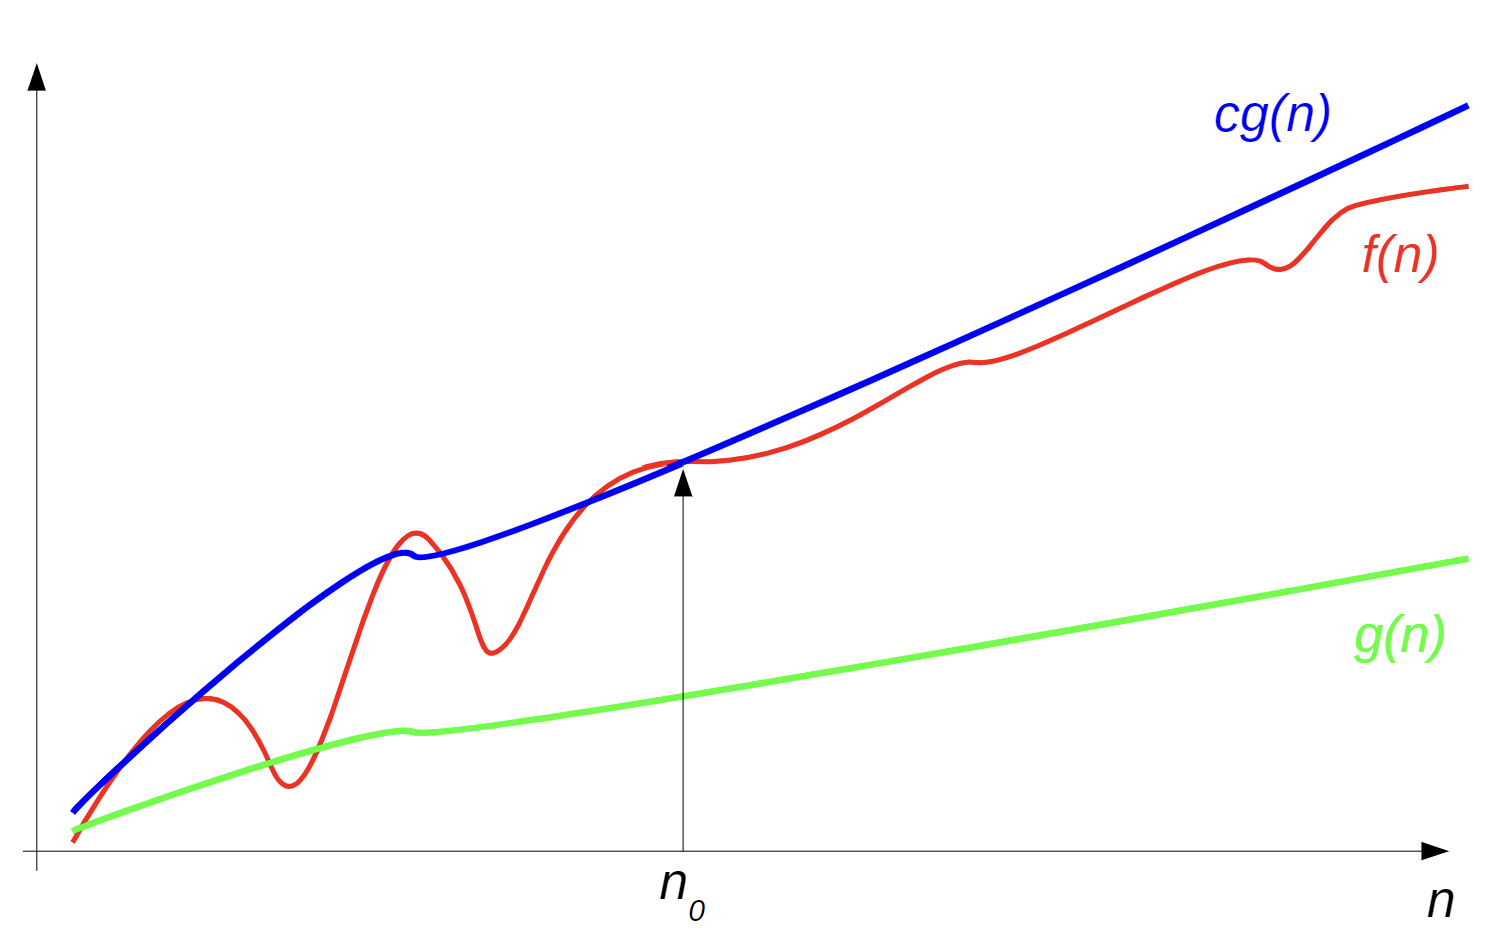
\includegraphics[width = 200px]{images/complexity_graph.png}
\end{center}
The values of $c$ and $n_0$ can be variable, and have any value, as long as the condition is fulfilled.\\
However, we are searching for $g(n)$ such that it refers to the smallest and simplest possible function of $n$ to allow for the existence of the values of $c$ and $n_0$ that will make the condition true.\\
A good strategy to select $c$ is the sum of the absolute values of all the coefficients in $f(n)$.\\
\textit{Note: $f(n)$ is equivalent to the $T(n)$ in the Time Complexity Analysis section.}\\
Another proof of $f(n)=O(g(n))$ is $\lim_{n \rightarrow \infty}\frac{f(n)}{g(n)}\neq \infty$.\\
For $g(n)$ to be useful, it should be simpler than $f(n)$ such as $1,n,n^2$, $n\log(n), 2^n, n!$.\\
However, once we go to exponential functions or above, the algorithms cease to be useful.
\end{document}